\chapter{2048と強化学習}
\label{chap:rl}
これまでに2048を対象とした強化学習の研究は数多くなされてきた. 
本章では強化学習の概要, および2048に対する強化学習の先行研究について記述する.

\section{強化学習の概要}
\label{sec:rl_general}
まず本節では2048との関係を踏まえつつ, 一般的な強化学習の概要について記述する.
なお本節の内容は全体に文献~\cite{Sutton1998}を参照して書かれた.

\subsection{マルコフ決定過程}
\label{subsec:mdp}
強化学習は与えられた環境において試行錯誤することを通して, 目標を達成するための戦略や意思決定を学習するための手法である.
学習や意思決定を行う主体はエージェントと呼ばれる.
エージェントは離散タイムステップに従って行動を選択し続け, 環境とやり取りを行う.

このような問題設定はマルコフ決定過程~(MDP)~というモデルによって定式化されている.
MDPは以下の$4$つの要素で構成される. 
\begin{itemize}
  \item 状態集合 $\mathcal{S}$
  \item 行動集合 $\mathcal{A}$
  \item 状態遷移関数$p:\mathcal{S} \times \mathcal{A} \times \mathcal{S} \rightarrow [0,1]$
  \item 報酬関数$r:\mathcal{S} \times \mathcal{A} \times \mathcal{S} \rightarrow \mathbb{R}$
\end{itemize}
エージェントはステップ$t$で状態$S_t \in \mathcal{S}$から行動$A_t \in \mathcal{A}$を選択する.
そして確率$p(S_{t+1}|S_t, A_t)$で次の状態$S_{t+1}$に遷移し, $R_{t+1} = r(S_t, A_t, S_{t+1})$を即時報酬として獲得する.
状態遷移関数と報酬関数は環境のダイナミクスと呼ばれることがある. 
図\ref{fig:mdp}にMDPの概念図を示す.
\begin{figure}[h]
  \centering
  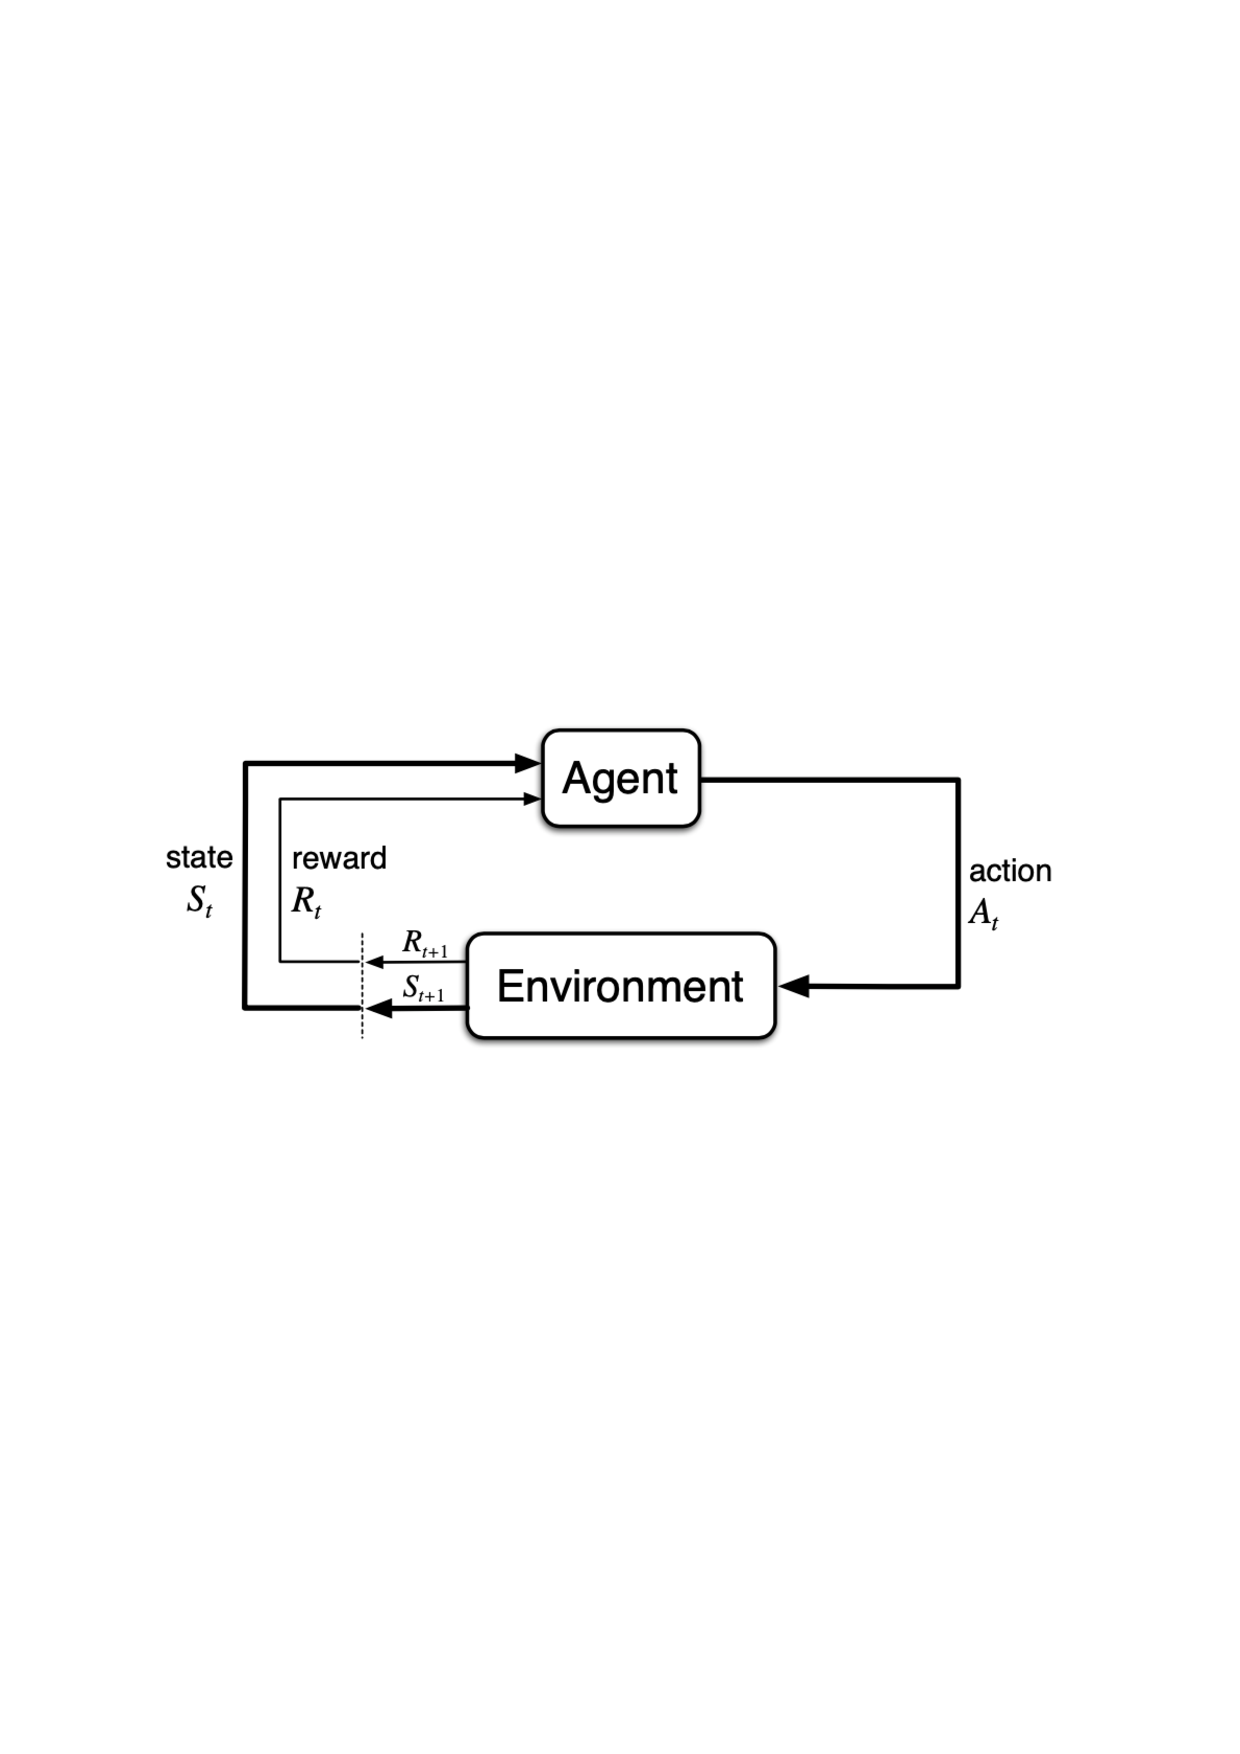
\includegraphics[width=\linewidth{}]{figures/MDP.pdf}
  \caption{MDPの模式図 (文献\cite{Sutton1998}より引用)}
  \label{fig:mdp}
\end{figure}

状態集合と行動集合が有限であるMDPを有限MDPと呼ぶ.
2048は有限MDPにそのまま当てはまるゲームである.
行動集合\textit{A}はプレイが選ぶ上下左右に対応し, 報酬はプレイヤが獲得する得点に直接対応する.

一般に強化学習で扱う問題には, エージェントと環境のやり取りが終わる終了状態が存在するepisodic taskと終了状態が存在しないcontinuing taskが存在する. 
episodic taskではエージェントと環境のやり取りを初期状態から終了状態までのエピソードと呼ばれる単位で分割することができる.
\ref{sec:property}節で説明したように2048は必ず終了するゲームであるため, 以降episodic taskでの定義を確認する. 

\subsection{方策と価値関数}
エージェントがある状態において行動を決定する際の戦略, すなわち確率分布$\pi:S \times A \rightarrow [0,1]$を方策と呼ぶ.
状態価値関数$v_{\pi}(s)$は状態$s$から方策$\pi$に従って行動を選択し続けた場合の累積報酬和の期待値であり, 次のように定義される.
\begin{align}
  v_{\pi}(s) \stackrel{\mathrm{def}}{=} \mathbb{E}_{\pi}\left[\sum_{k=0}^T R_{t+k+1}|S_t=s \right]
\end{align}
同様に状態$s$から行動$a$を選択し, その後方策$\pi$に従って行動を選択し続けた場合の累積報酬和の期待値である行動価値関数$q_{\pi}(s,a)$の定義は以下のようになる.
\begin{align}
  q_{\pi}(s,a) \stackrel{\mathrm{def}}{=} \mathbb{E}_{\pi}\left[\sum_{k=0}^T R_{t+k+1}|S_t=s, A_t=a \right]
\end{align}

強化学習の目標は多くの報酬を獲得できるような良い方策を見つけることである.
価値関数の定義より2つの方策$\pi$と$\pi'$があるとすると, すべての状態$s \in S$について$v_\pi(s) \geq v_{\pi'}(s)$が成り立つならば$\pi$は$\pi'$と等価か$\pi'$よりも良い方策だと言える.
ここで他のすべての方策と比べて等価であるか, それよりも良い方策が少なくとも$1$つ存在する.
これは最適方策$\pi_*$と呼ばれる方策である.
$\pi_*$に従うときの状態価値関数は最適状態価値関数と呼ばれ, $v_*$で表される.
同様に$\pi_*$に従うときの行動価値関数は最適行動価値関数と呼ばれ, $q_*$で表される.
それぞれの具体的な定義を式~\ref{eq:v_opt}, \ref{eq:q_opt}に示す.
\begin{align}
  \label{eq:v_opt}
  v_*(s) &= \max_\pi v_{\pi}(s) \quad \text{for all } s \in S \\
  \label{eq:q_opt}
  q_*(s,a) &= \max_\pi q_{\pi}(s, a) \quad \text{for all } s \in S \text{ and } a \in A(s)
\end{align}
このとき$v_*(s) = \max_{a \in A(s)} q_*(s, a)$であるから, 以下の式が導かれる~(図~\ref{fig:backup}を参照)~.
\begin{align}
  v_*(s) &= \max_{a \in A(s)} q_*(s, a) \\
  \label{eq:bellman_v_opt}
               &= \max_{a \in A(s)} \mathbb{E}[R_{t+1} + v_*(S_{t+1}) | S_t=s, A_t=a] \\
  q_*(s, a) &= \mathbb{E}[R_{t+1} + v_*(S_{t+1}) | S_t=s, A_t=a] \\
  \label{eq:bellman_q_opt}
                  &= \mathbb{E}[R_{t+1} + \max_{a'} q_*(S_{t+1}, a') | S_t=s, A_t=a]
\end{align}
式~\ref{eq:bellman_v_opt}, \ref{eq:bellman_q_opt}はベルマン最適方程式と呼ばれる.
\begin{figure}[h]
  \centering
  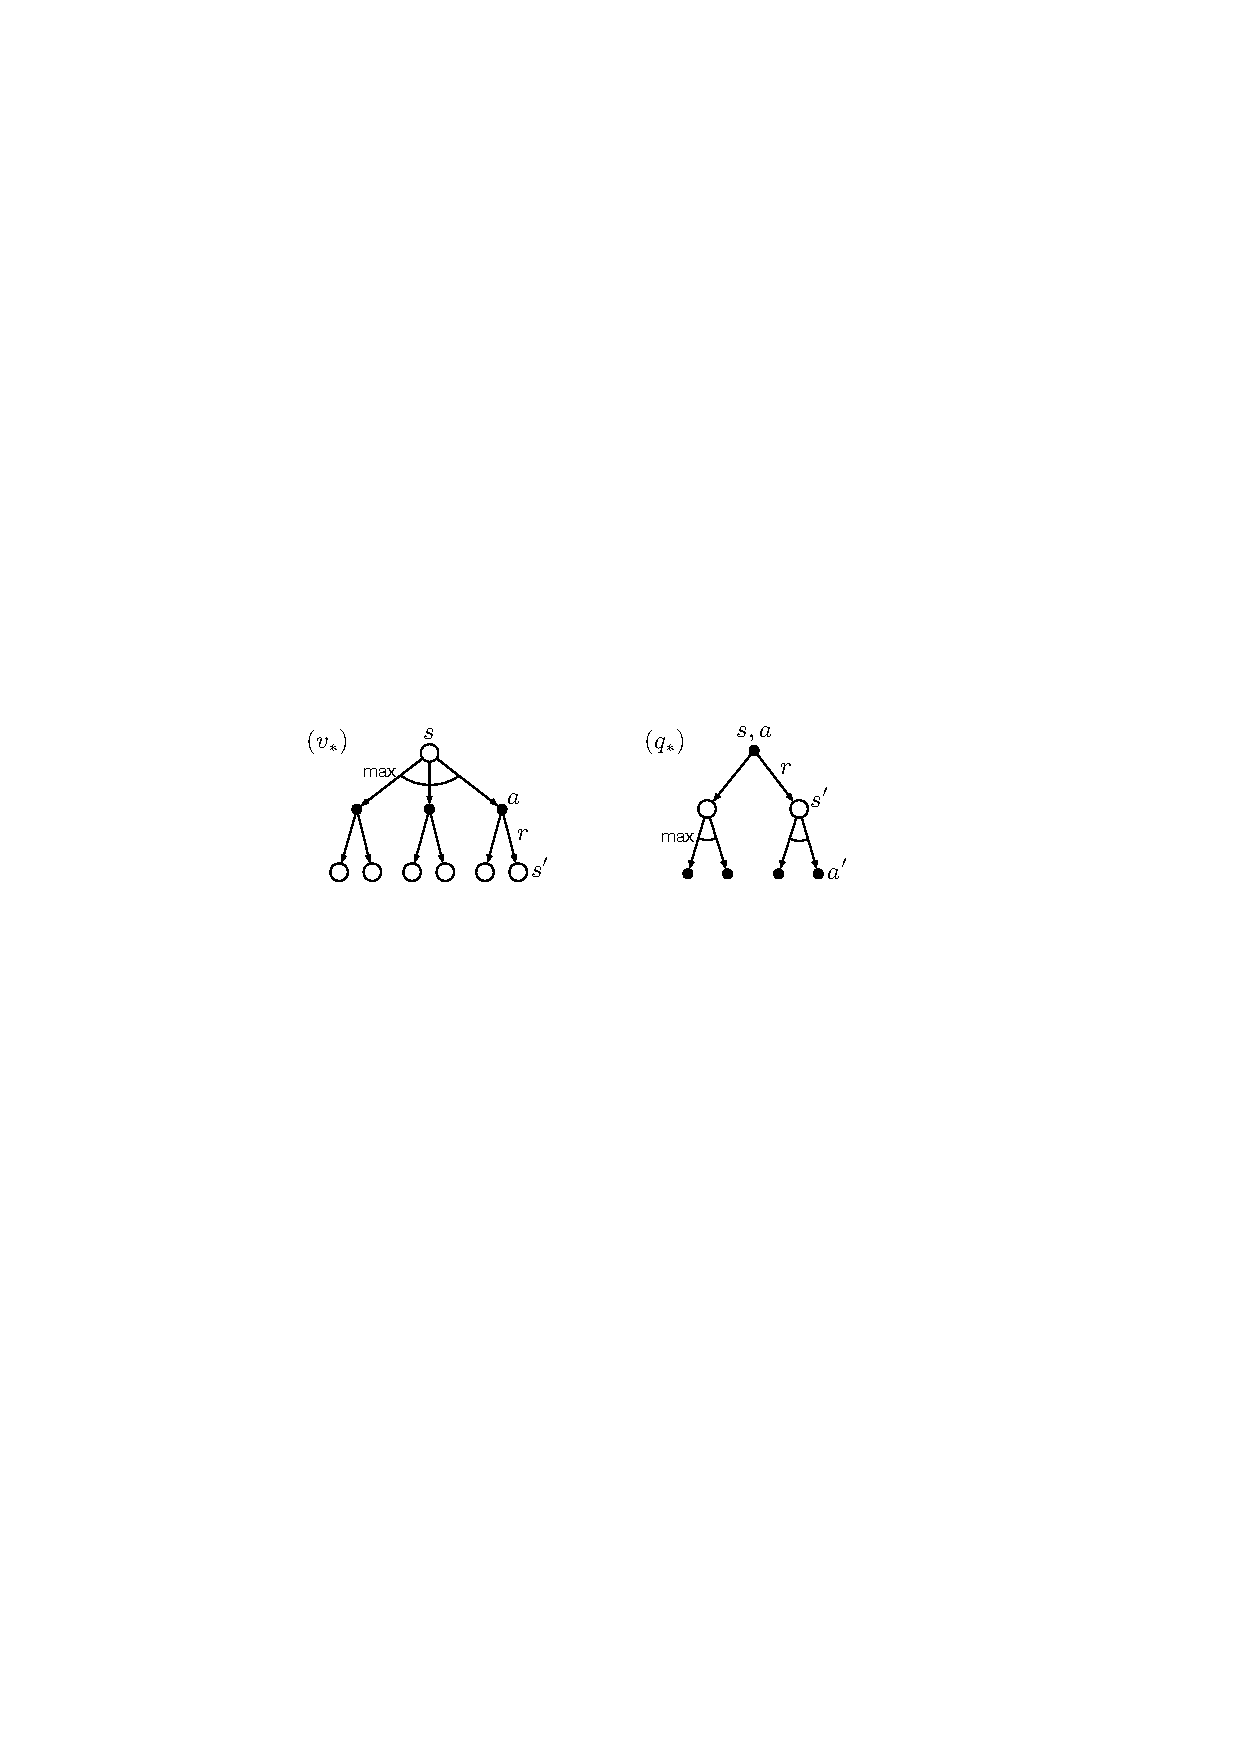
\includegraphics[width=\linewidth{}]{figures/backup.pdf}
  \caption{最適価値関数のバックアップ図 (文献\cite{Sutton1998}より引用)}
  \label{fig:backup}
\end{figure}

\subsection{価値ベースな手法}
状態$s$における最適方策に従った具体的な行動は$\argmax \mathbb{E}[R_{t+1} + v_*(S_{t+1}) | S_t=s, A_t=a]$と, $1$ステップ先の状態を探索してそれらの最適状態価値関数を参照することで計算できる.
最適行動価値関数が参照できれば, $1$ステップ先の状態を探索する必要すらなく, 単に$\argmax q_*(s, a)$を選択すればよい.
最適方策を得るために価値関数を学習する手法は価値ベースな手法と呼ばれる.

Q学習は最も基本的な価値ベースな手法の$1$つで, 最適行動価値関数$q_*$の推定値$Q$を得られた経験から学習する.
状態$S_t$から行動$A_t$を選択し, 報酬$R_{t+1}$を獲得して次の状態$S_{t+1}$に遷移したとする.
このときQ学習は以下の更新式~\ref{eq:q_learning}に従って$Q(S_t, A_t)$を更新する.
\begin{align}
  \label{eq:q_learning}
  Q(S_t, A_t) \leftarrow Q(S_t, A_t) + \alpha [R_{t+1} + \max_a Q(S_{t+1}, a) - Q(S_t, A_t)] 
\end{align}
式~\ref{eq:q_learning}は現在の推定値$Q(S_t, A_t)$を, ベルマン最適方程式~\ref{eq:bellman_q_opt}の右辺の推定値である$R_{t+1} + \max_a Q(S_{t+1}, a)$に近づけていると解釈できる.
任意の$(s, a) \in \mathcal{S} \times \mathcal{A}$について$Q(s,a)$が更新され続けるという条件の下で, Q学習は収束が保証されている.

状態集合や行動集合が大きい場合や有限でない場合には, テーブル形式でQ値を保持することができないため何らかの関数近似を行う必要がある.
近年では深層学習~\cite{DeepLearning}の研究の発展により, 関数近似の方法としてニューラルネットワークが用いられることが多い.
価値関数や方策をニューラルネットワークで近似する手法は, まとめて深層強化学習と呼ばれる.

Q値をニューラルネットワークで近似する, Deep Q Network~(DQN)~\cite{DQN}は深層強化学習の先駆けとして有名な手法である. 
DQNはエージェントが蓄積したデータからバッチサイズ個をランダムにサンプルし, これらをニューラルネットワークの学習に使用するExperience Replayを提案した.
Experience Replayによって学習データは適度にばらつき, ニューラルネットワークの学習は安定化する.
Schaulらが提案したPrioritized Experience Replay~\cite{prioritized}は一様ランダムではなく, priorityという重みに従ってデータをサンプルするExperience Replayである.
優先的に学習したいデータを積極的に訓練に用いることで, 学習効率が上がることが期待される.
価値ベースな深層強化学習手法はDQNの発表以降, 様々な工夫が提案され続けている.
詳細は文献~\cite{deepRL}の$4$節などを参照されたい.

\subsection{方策ベースな手法}
方策を直接パラメタライズされた関数で近似し, パラメータを学習する手法を全般に方策ベースな手法と呼ぶ.
なお方策ベースな手法においても価値関数の学習を行うことはあるが, 良い方策のパラメータを学習するために必要とするものであり, 直接的な行動の選択には関与しない.

方策のパラメータ$\pmb{\theta}$は目的関数$J(\pmb{\theta})$を最大化するように更新される.
$J(\pmb{\theta})$は, 方策$\pi_{\pmb{\theta}}$に従ったときの初期状態$s_0$の価値$v_{\pi_{\pmb{\theta}}}(s_0)$と定義することができる.
このとき方策$\pi$のもとで状態$s$を訪れる確率を$\mu(s)$とすると, $\nabla J(\pmb{\theta})$は以下の方策勾配定理によって求めることができる.
\begin{align}
  \label{eq: policy_gradient_theorem}
  \nabla J(\pmb{\theta}) \propto \sum_s \mu(s) \sum_a q_{\pi}(s,a) \nabla \pi(a|s, \pmb{\theta})
\end{align}
さらに以下のように変形する.
\begin{align}
  \nabla J(\pmb{\theta}) &\propto \sum_s \mu(s) \sum_a q_{\pi}(s,a) \nabla \pi(a|s, \pmb{\theta}) \notag \\
  & = \mathbb{E}_{\pi} \left[\sum_a q_\pi(S_t, a) \nabla \pi(a|S_t, \pmb{\theta})\right] \notag \\
  & = \mathbb{E}_{\pi} \left[\sum_a \pi(a|S_t, \pmb{\theta}) q_\pi(S_t, a) \frac{\nabla \pi(a|S_t, \pmb{\theta})}{\pi(a|S_t, \pmb{\theta})}\right] \notag \\
  & = \mathbb{E}_{\pi} \left[q_\pi(S_t,A_t) \frac{\nabla \pi(A_t|S_t, \pmb{\theta})}{\pi(A_t|S_t,\pmb{\theta})}\right] \notag \\
  & = \mathbb{E}_{\pi} \left[q_\pi(S_t,A_t) \nabla \ln \pi(A_t|S_t, \pmb{\theta}) \right] \notag \\
\end{align}
よって学習率を$\alpha$とすると, パラメータ$\pmb{\theta}$の更新式が導かれる.
\begin{align}
  \label{eq:reinforce}
  \pmb{\theta}_{t+1} \leftarrow \pmb{\theta}_{t} + \alpha \left[q_\pi(S_t,A_t) \nabla \ln \pi(A_t|S_t, \pmb{\theta}) \right]
\end{align}
ただし未知の値$q_\pi(S_t,A_t)$を, 学習データから推定する必要がある.
Williams~\cite{Williams:92}は$q_\pi(S_t,A_t)$の推定値として, $S_t$から$A_t$を選択して実際に獲得した報酬の総和$G_t = \Sigma_{k=0}^{T} R_{t+k+1}$を用いることを提案した.
$G_t$は$q_\pi(S_t,A_t)$の不偏推定量としての性質をみたす一方で, 分散が大きく学習が安定しない.
またパラメータの更新をエピソードが終了するまで行うことができない.

ここで式~\ref{eq: policy_gradient_theorem}において, 行動$a$に依存しない定数を$b(s)$として$\Sigma_a b(s) \nabla \pi(a|s,\pmb{\theta}) = b(s) \nabla \Sigma_a \pi(a|s, \pmb{\theta}) = 0$に注目すると, 以下の式~\ref{eq:reinforce_baseline}が成り立つ.
\begin{align}
  \label{eq:reinforce_baseline}
  \nabla J(\pmb{\theta}) \propto \sum_s \mu(s) \sum_a \left(q_{\pi}(s,a) - b(s)\right) \nabla \pi(a|s, \pmb{\theta})
\end{align}
$b(s)$として$s$の価値関数$v_{\pi}(s)$を考えることが一般的である.
$q_{\pi}(s,a) - v_{\pi}(s)$は, 状態$s$で行動$a$をとることが他の行動をとることに比べて, どれくらい良いかを示す値で一般的にアドバンテージと呼ばれる.
よってパラメータ更新式~\ref{eq:reinforce}中の$q_\pi(S_t,A_t)$の代わりに, アドバンテージ$q_\pi(S_t,A_t) - v(S_t)$を推定する.
そのために方策関数の学習と同時に, 価値関数$v_\pi$の推定値$V$を学習する.
$q_\pi(S_t,A_t) = \Sigma_{k=0}^{n-1} R_{t+k+1} + v_\pi(S_{t+n})$であるから, 以下の方策パラメータ$\pmb{\theta}$の更新式~\ref{eq:actor_critic}が導かれる.
\begin{align}
  \label{eq:actor_critic}
  \pmb{\theta}_{t+1} \leftarrow \pmb{\theta}_{t} + \alpha \left[\sum_{k=0}^{n-1} \big(R_{t+k+1} + V(S_{t+n}) - V(S_{t+n})\big) \nabla \ln \pi(A_t|S_t, \pmb{\theta}) \right]
\end{align}
ここで$\Sigma_{k=0}^{n-1} R_{t+k+1} + v_\pi(S_{t+n})$は$n$ステップリターンと呼ばれる.
$n$をエピソードの終了時刻$T$とすると, $n$ステップリターンは$G_t$に一致する.
このように学習した価値関数を行動の良さを評価するために用いる手法は, 全般にactor-criticな手法と呼ばれる.

Mnihら~\cite{A3C}が提案したasynchronous advantage actor-critic~(A3C)~は, 方策関数と価値関数をニューラルネットワークにより近似したactor-criticな手法で, Atariや物理シミュレーションの実験で高い成果を収めた.
A3Cの発表以降, 方策ベースな深層強化学習の研究は数多くなされている.
特にSchulmanらが提案したProximal Policy Optimization~(PPO)~\cite{PPO}は有名手法の$1$つである.
PPOは方策の急激な更新を抑えるように工夫した手法で, 学習の安定性と実装のしやすさから現在でも多くの分野で用いられている.

\subsection{AlphaZeroとMuZero}
\label{subsec:zero}
Silverらが提案したAlphaZero~\cite{AlphaZero}は, 囲碁やチェスなどの二人零和完全確定情報ゲームを対象とした有力な深層強化学習手法である.
AlphaZeroは盤面の特徴量を入力として, その盤面における方策と価値を出力するニューラルネットワークを持つ.
これをモンテカルロ木探索~(MCTS)~による自己対戦を通して得たデータから学習する.
そのため人間の棋譜などの教師データを使うことなく, 囲碁, 将棋, チェスにおいて当時の有力なプログラムを上回る強さを示して注目を集めた.

AlphaZeroはMCTSを行うにあたって, ゲームのルールや環境のダイナミクスが既知であることを前提としている.
すなわち現在の状態$s_t$から行動$a_t$を選択した後の状態$s_{t+1}$を, $s_t$のみ観測している状況から知ることができる必要がある.
そのためAlphaZeroは複雑なダイナミクスを持つAtariなどのゲームには適用することが難しい.
Schrittwieserらが提案したMuZero~\cite{MuZero}は, ニューラルネットワークで環境のダイナミクスをモデル化し, 学習することを提案した.
MuZeroは二人零和完全確定情報ゲームにおいてAlphaZeroと同等の強さ, Atariにおいて当時の有力手法と同等以上の性能を示した.
\ref{subsec: stochastic_muzero}節でMuZeroを確率的な環境に対応できるように拡張した, Stochastic MuZeroについて述べる.
そこでMCTSの具体的な方法や, ニューラルネットワークの学習方法について述べる.

\section{2048への強化学習の応用}
\label{sec:rlto2048}
\ref{sec:rl_general}節では強化学習一般の概要について説明した.
これを踏まえて本節では, 2048を対象とした強化学習研究の先行研究について概説する.

\subsection{TD afterstate学習}
\label{subsec: td_afterstate}
Szubertら~\cite{Szubert}はTD afterstate学習と呼ばれる価値ベースの強化学習手法を提案した.
2048はゲームの性質上, 状態$s$から行動$a$をとって獲得する得点$r(s,a)$と遷移するafterstate $s'$は決定的である.
よってafterstate $s'$の最適価値を$v_*'(s')$と表すと, 行動価値$q_*(s,a)$は$q_*(s,a) = r(s,a) + v_*'(s')$と分解できる.
そこでTD afterstate学習は, Q値ではなくafterstateの価値$v_*'$の推定値$V'$を式~\ref{eq:td_afterstate}に従って更新する.
\begin{align}
  \label{eq:td_afterstate}
  V'(S_{t}^{'}) \leftarrow  V'(S_{t}^{'}) + \alpha [R_{t+1} + V'(S_{t+1}^{'}) - V'(S_{t}^{'})]
\end{align}
式~\ref{eq:td_afterstate}はQ学習の更新式~\ref{eq:q_learning}において, $Q(S_t, A_t) = R(S_t, A_t) + V'(S_{t}^{'})$として書き直したものと見ることができる.

SzubertらはN-tupleネットワークというヒューリスティックな盤面評価関数を用いて$V'$を表現し, $2048$のタイルを$98$\%の確率で到達させることに成功した.
Jaskowski~\cite{DBLP:journals/corr/Jaskowski16}はこれに様々な工夫を加えた学習方法を提案し, 最終的にexpectimax探索を$1$手$1$秒の制限で行うことで平均$609,104$点を獲得するプレイヤを開発した.
松崎~\cite{KiminoriMatsuzaki2021}はニューラルネットワークによって表現した$V'$を学習させ, $3$-ply expectimax探索を行うことで平均$406,927$点を達成した.

Szubertらは文献~\cite{Szubert}でN-tupleネットワークを用いたQ学習の実験も行ったが, TD afterstate学習の性能を大きく下回る結果になったことを報告している.
TD afterstate学習は観測している状態$s$からafterstate $s'$への遷移までをシミュレートする, いわば$0.5$手読みの探索を行っているため, $0$手読みのQ学習と比べて学習しやすいと考えられる.

\subsection{Afterstate PPO}
\ref{subsec: td_afterstate}節では, 価値ベースな手法であるTD afterstate学習が2048において主流な強化学習手法の$1$つであることを説明した.
一方で, 2048において目立った方策ベースな強化学習手法は
山下ら~\cite{afterstate_ppo}はPPO~\cite{PPO}を2048に工夫して適用する, Afterstate PPOという手法を提案した.
すなわち状態$s$から行動$a$をとったときのafterstateをニューラルネットワークの入力とし, その出力を行動$a$の選択確率のロジットとする.
通常のPPOでは全く学習が進まなかった一方で, Afterstate PPOは学習後2048のタイルを平均約$50\%$の割合で完成させることに成功した.

\subsection{Stochastic MuZero}
\label{subsec: stochastic_muzero}
Antonoglouらが提案したStochastic MuZero~\cite{StochasticMuZero}は~\ref{subsec:zero}節で述べたMuZeroを, 確率的な環境にも対応できるように拡張した手法である.
Stochastic MuZeroは確率的ゲームである2048とバックギャモンでMuZeroを大きく上回るパフォーマンスを発揮した.
さらにランダム性のない囲碁においてもMuZeroと同等のレーティングを達成し, 対象とするドメインが幅広いことを示した.
2048においては, \ref{subsec: td_afterstate}節で述べたTD afterstate学習の先行研究~\cite{DBLP:journals/corr/Jaskowski16}と比較して, 一切のドメイン知識を必要とせず, より優れたパフォーマンスを出したことが強調された.
一方で, 論文内で示されたStochastic MuZeroの最終的な平均スコアは約$50$万点で, expectimax探索を行うことで平均$609,104$点を達成した文献~\cite{DBLP:journals/corr/Jaskowski16}の結果を明確に上回るとはいえない.

Stochastic MuZeroは方策・価値ニューラルネットワークに加えて, 環境のダイナミクスモデルをニューラルネットワークにより推論する.
これらのニューラルネットワークを, モンテカルロ木探索~(MCTS)~によるプランニングを行って得た学習データを用いて訓練する.
以下ではAlphaZeroのように, 環境のダイナミクスを既知とした場合におけるStochastic MuZeroの方法を, 2048に適用することを想定して具体的に説明する.
説明の便宜上これを本稿では, 2048-AlphaZeroと呼ぶことにする.
2048-AlphaZeroはMCTSの実行方法, 方策・価値ニューラルネットワークの学習方法については, Stochastic MuZeroと全く同一である.
Stochastic MuZeroの環境のダイナミクスモデルの学習方法については, 文献~\cite{StochasticMuZero}の$4$節を参照されたい.

\subsubsection*{2048-AlphaZeroのMCTS}
\label{subsubsec:mcts}
2048-AlphaZeroは$2$つのニューラルネットワークを持つ.
$1$つ目は, 状態盤面$s$の特徴量を入力として$s$における方策, $s$の価値を出力するニューラルネットワーク$f$である.
$2$つ目は, afterstate盤面$s'$の特徴量を入力として$s'$の価値を出力するニューラルネットワーク$g$である.
これら$2$つのニューラルネットワーク$f$と$g$を用いてMCTSを実行する.

\ref{sec:rule}節で述べたように, 2048は状態とafterstateという$2$種類の盤面が交互に繰り返される.
そのため2048-AlphaZeroはMCTSにおいて, それぞれに対応するdecisionノードとchanceノードという$2$種類のノードから成る探索木を用いる.
探索木中のそれぞれのノード$s$は, 以下の$5$つの統計量を管理する.
\begin{itemize}
  \item $N(s) \cdots$探索中に$s$を訪問した回数
  \item $W(s) \cdots$ $s$を根とする部分木中のノードの価値の推定値の合計
  \item $Q(s) \cdots$ $s$を根とする部分木中のノードの価値の推定値の平均~($W(s) / N(s)$)
  \item $P(s) \cdots$ $s$の親から$s$への遷移確率
  \item $R(s) \cdots$ $s$の親から$s$へ遷移するときに獲得する即時報酬~(得点)
\end{itemize}
探索木は最初, 現在の盤面~(状態)~に対応するdecisionノード$s_0$のみから成る.
MCTSは選択, 評価, 逆伝播, 展開の$4$つのステップを繰り返すことで, $s_0$を根とする探索木を大きくする.
この$4$つのステップはまとめてシミュレーションと呼ばれる.
シミュレーションを繰り返すことで深い探索を行い, 良い行動を選択することができる.
以下ではそれぞれのステップについて説明する.

\paragraph{選択}
探索木の根ノード$s_0$~(decisionノード)~から有望な子ノードを選択し, これを葉ノード$s_L$に至るまで辿り続ける.
decisionノード$s_d$においては, 以下のPUCT式~\ref{eq:puct}が最大となるような子chanceノード$s_c$を選択する.
\begin{align}
  Q(s_c) + C(s_c)P(s_c)\frac{\sqrt{1+N(s_d)}}{1+N(s_c)}
  \label{eq:puct}
\end{align}
ただし$C(s_c)$は探索率を表す.
これは現段階での価値の推定値$Q(s_c)$と探索項$C(s_c)P(s_c)\sqrt{1+N(s_d)}/(1 + N(s_c))$を合計したものである.
$N(s_c)$が小さい子chanceノードほど探索項は大きな値を示す.
一方chanceノード$s_c$においては, 単にそれぞれの子decisionノード$s_d$への遷移確率$P(s_d)$に従って確率的に選択する.

\paragraph{評価~(図~\ref{fig:evaluate})}
選択のステップの葉ノード$s_L$をニューラルネットワークにより評価する.
$s_L$がdecisionノードである場合には, $s_L$に対応する状態における, 方策$\pi(\cdot|s_L)$および価値を$v_L$を$f$で評価することで得る.
$s_L$がchanceノードである場合には, $s_L$に対応するafterstateの価値$v_L$のみを$g$で評価することで得る.

\paragraph{展開~(図~\ref{fig:expand})}
$s_L$がdecisionノードである場合には, $s_L$に対応する状態から遷移可能なafterstateを$s_L$の子chanceノードとして探索木に追加する.
それぞれの子chanceノード$s_c$について, $P(s_c) = \pi(s_c|s_L)$とする.

$s_L$がchanceノードである場合には, $s_L$に対応するafterstateから遷移可能な状態を$s_L$の子decisionノードとして探索木に追加する.
それぞれの子decisionノード$s_d$について, $P(s_d)$は$s_L$に対応するafterstateから$s_d$に対応する状態へ遷移する環境が与える確率とする.

\paragraph{逆伝播~(図~\ref{fig:backpropagate})}
$s_L$について, $N(s_L)=0, W(s_L)=0, Q(s_L)=0$と初期化する.
さらに$s_L$から$s_0$に至る各ノード$s_t$について, 以下のように各統計量の値を更新する.
\begin{align*}
  N(s_t) &\leftarrow N(s_t) + 1 \\
  W(s_t) &\leftarrow W(s_t) + \Sigma_{k=t+1}^{L} R(s_k) + v_L \\
  Q(s_t) &\leftarrow \frac{W(s)}{N(s)}
\end{align*}

\begin{figure}
  \begin{subfigure}[T]{0.4\columnwidth}
    \centering
    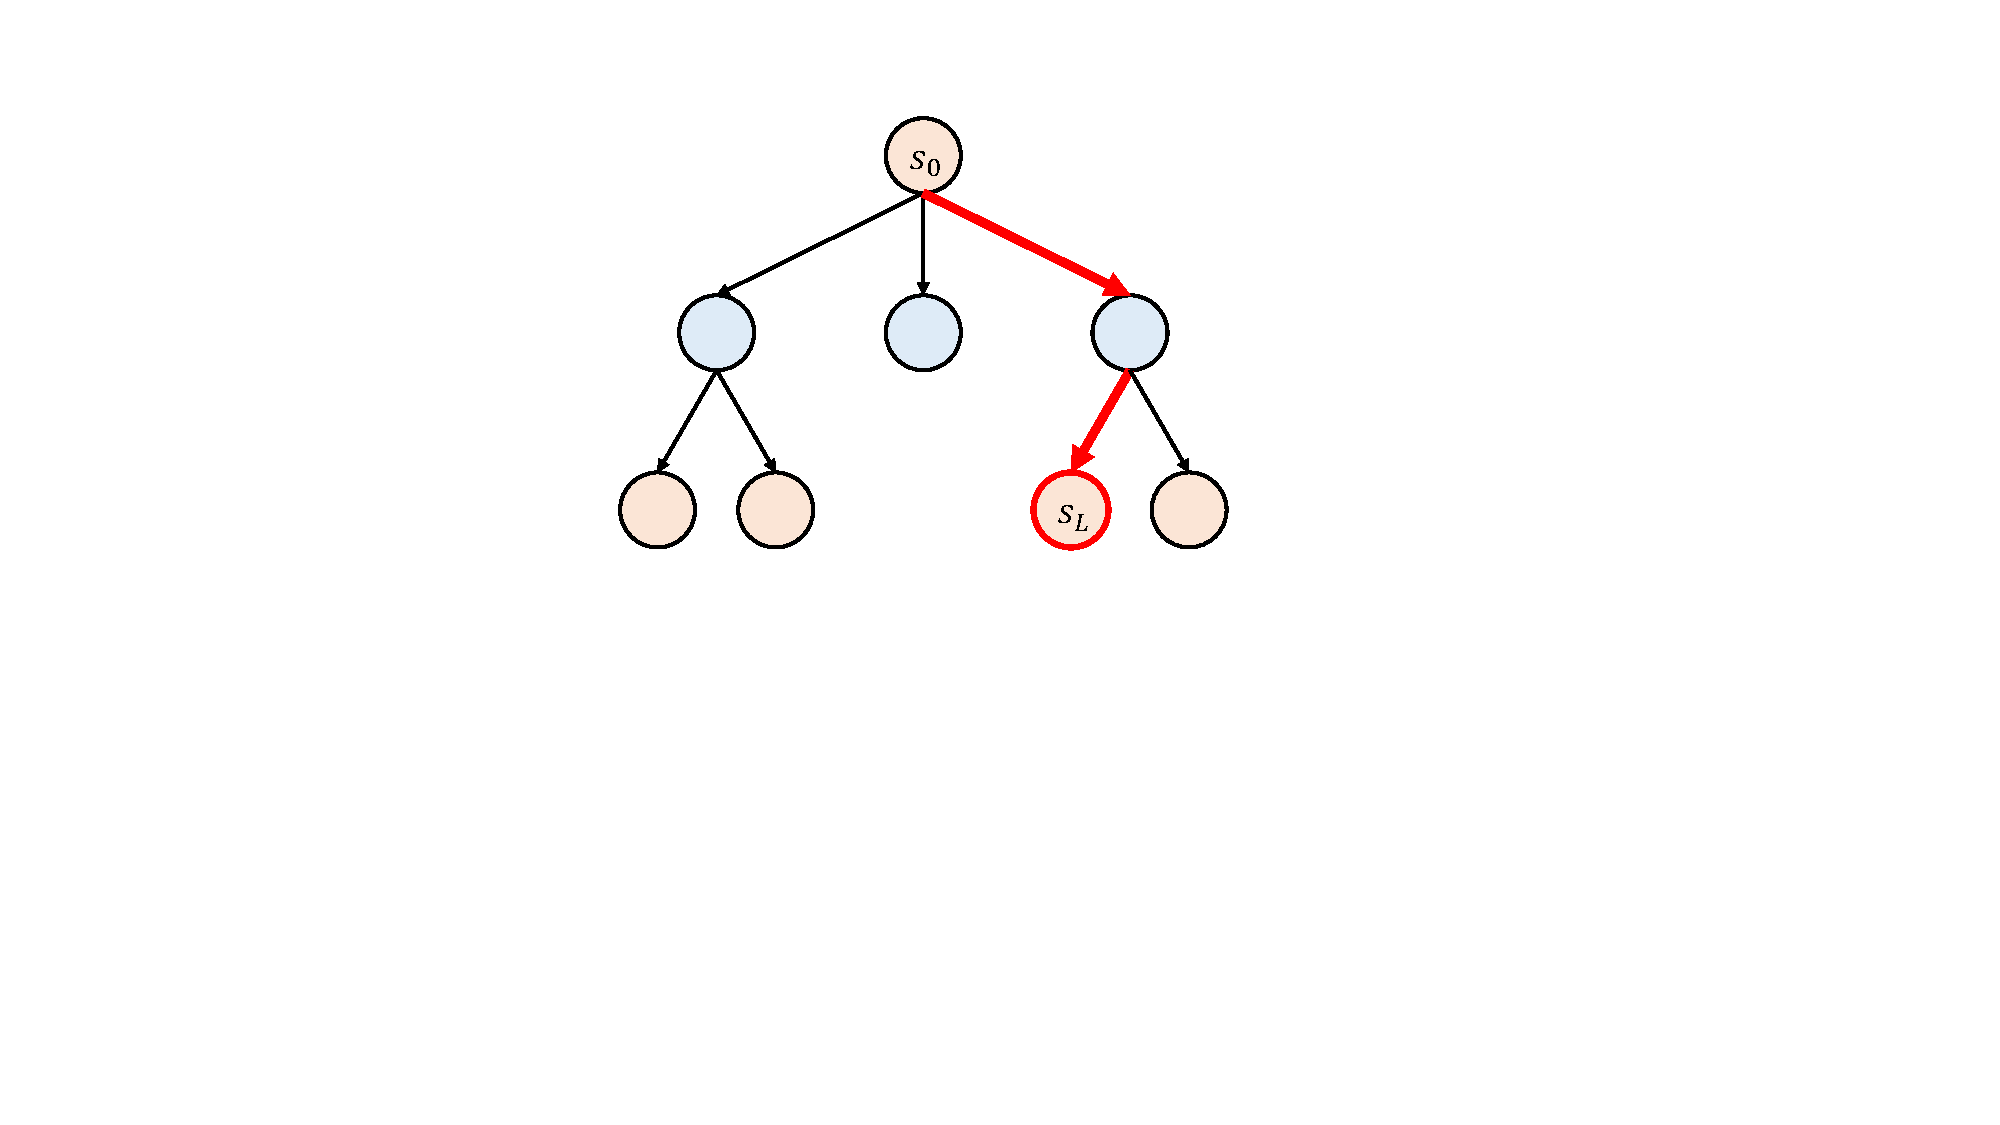
\includegraphics[width=\columnwidth]{figures/selection_.pdf}
    \caption{選択}
    \label{fig:selection}
  \end{subfigure}
  \begin{subfigure}[T]{0.4\columnwidth}
    \centering
    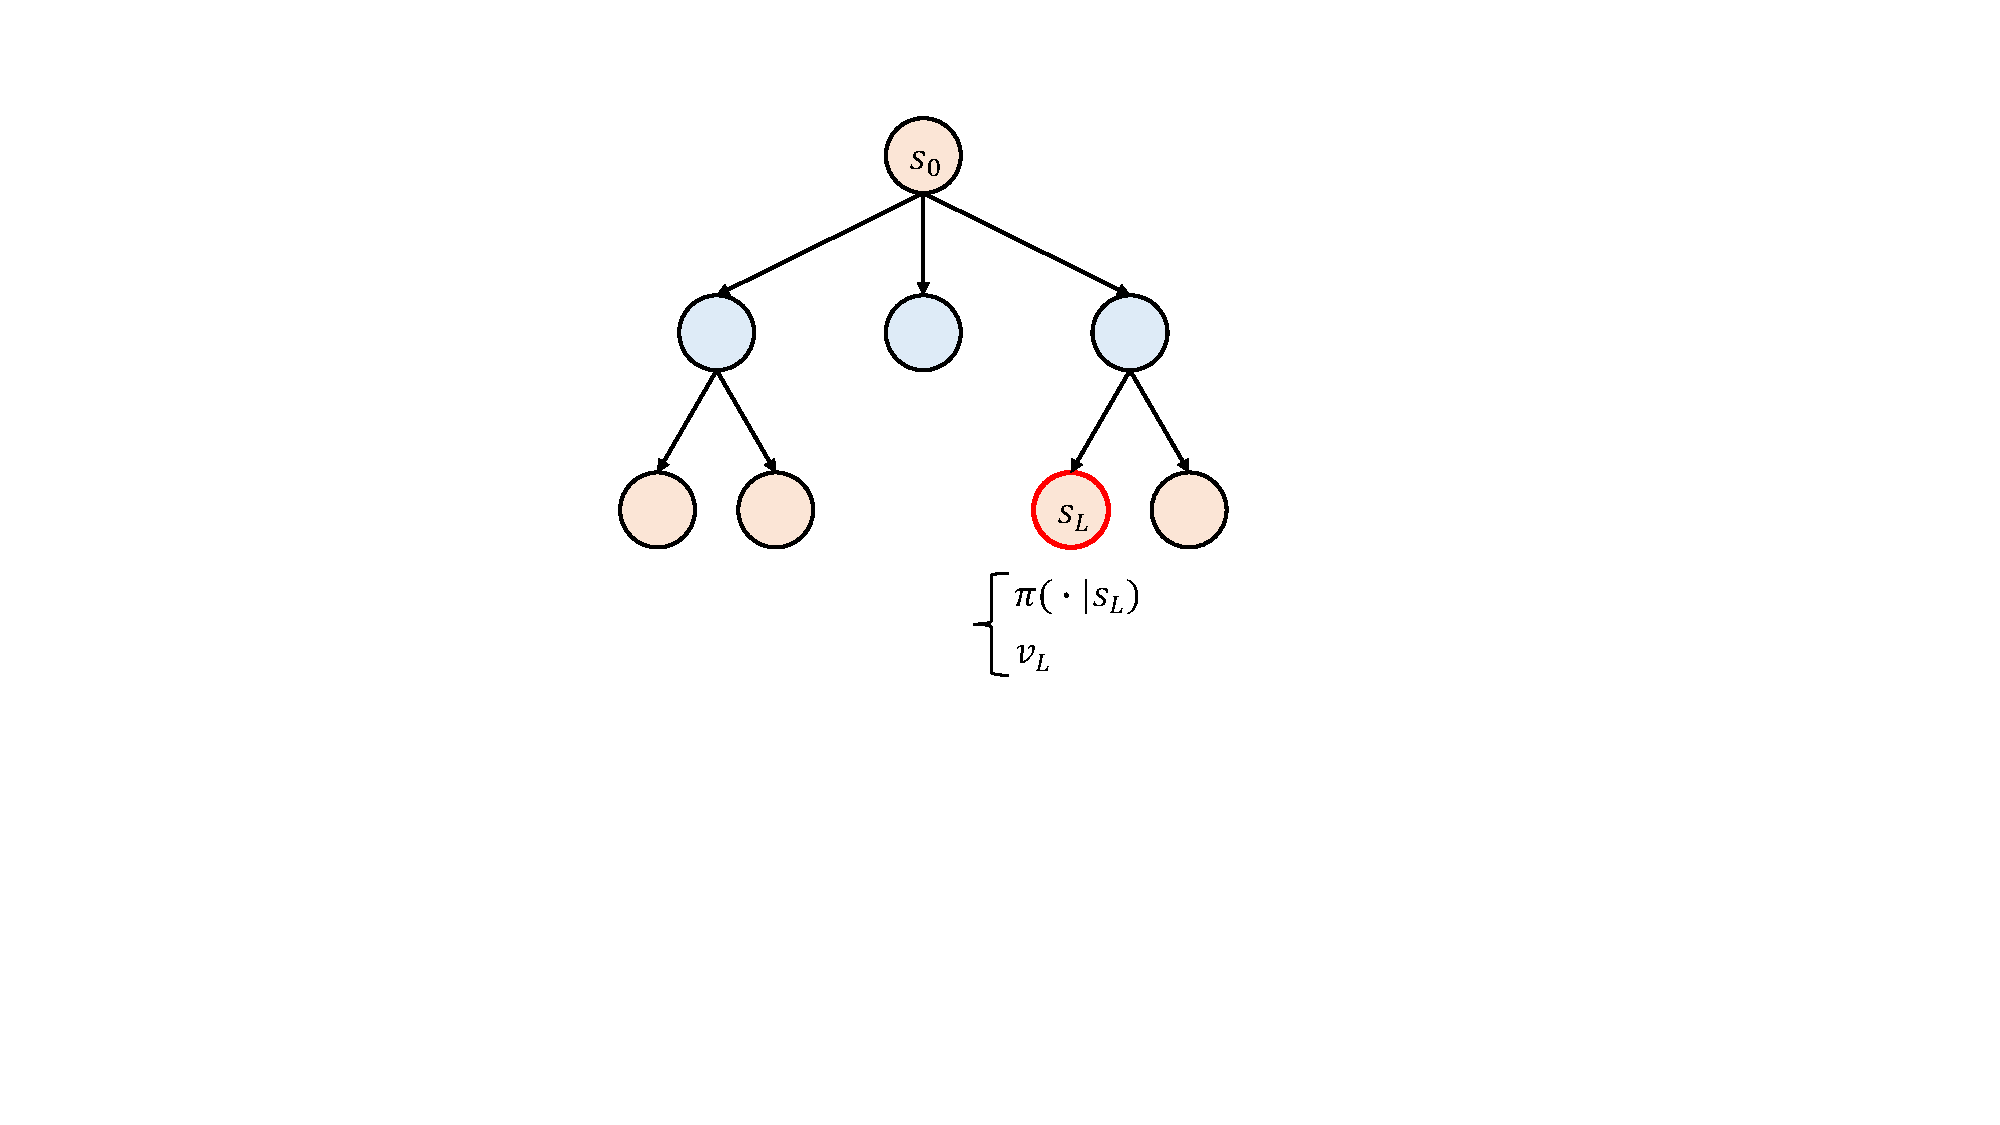
\includegraphics[width=\columnwidth]{figures/evaluate_.pdf}
    \caption{評価}
    \label{fig:evaluate}
  \end{subfigure}
  \begin{subfigure}[T]{0.4\columnwidth}
    \centering
    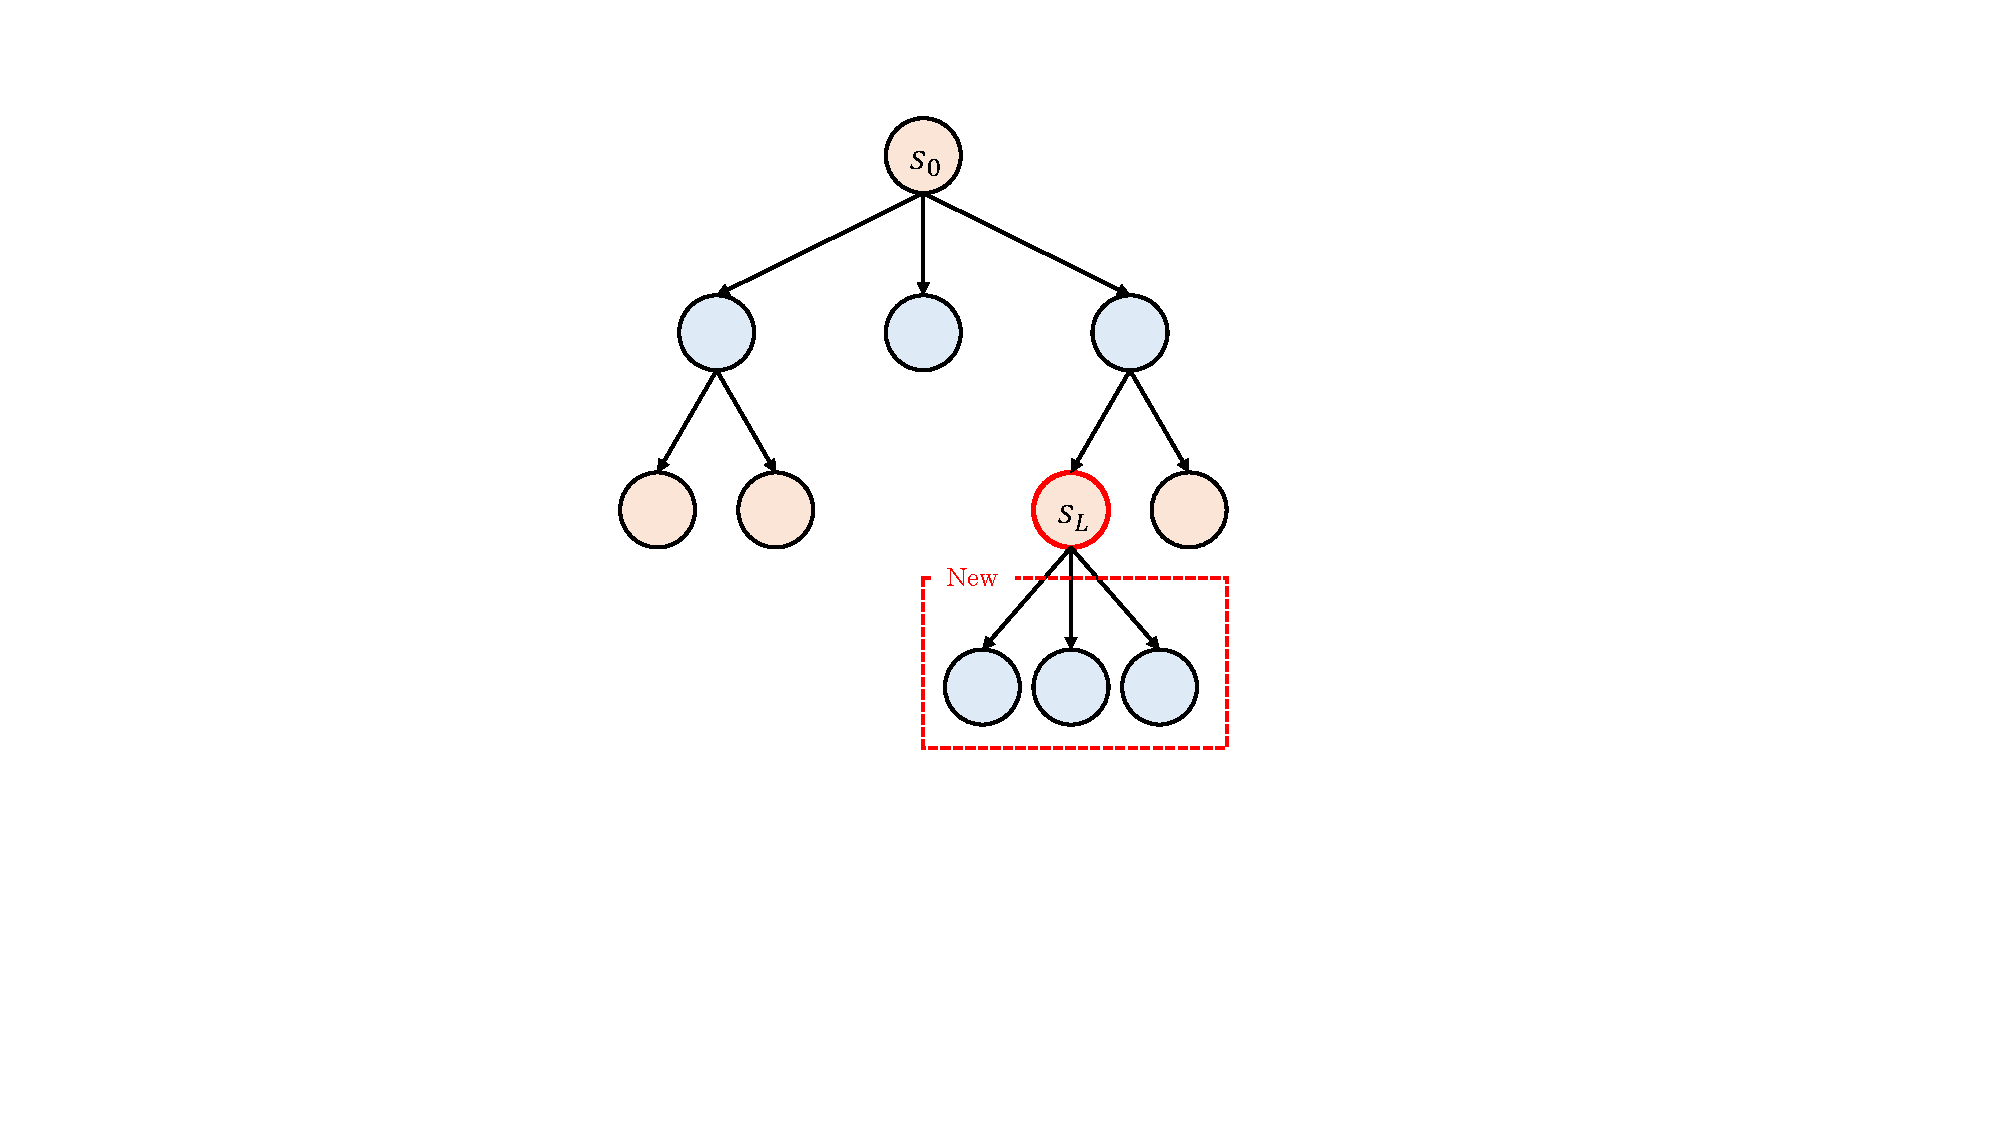
\includegraphics[width=\columnwidth]{figures/expand_.pdf}
    \caption{展開}
    \label{fig:expand}
  \end{subfigure}
  \hspace{3cm}
  \begin{subfigure}[T]{0.4\columnwidth}
    \centering
    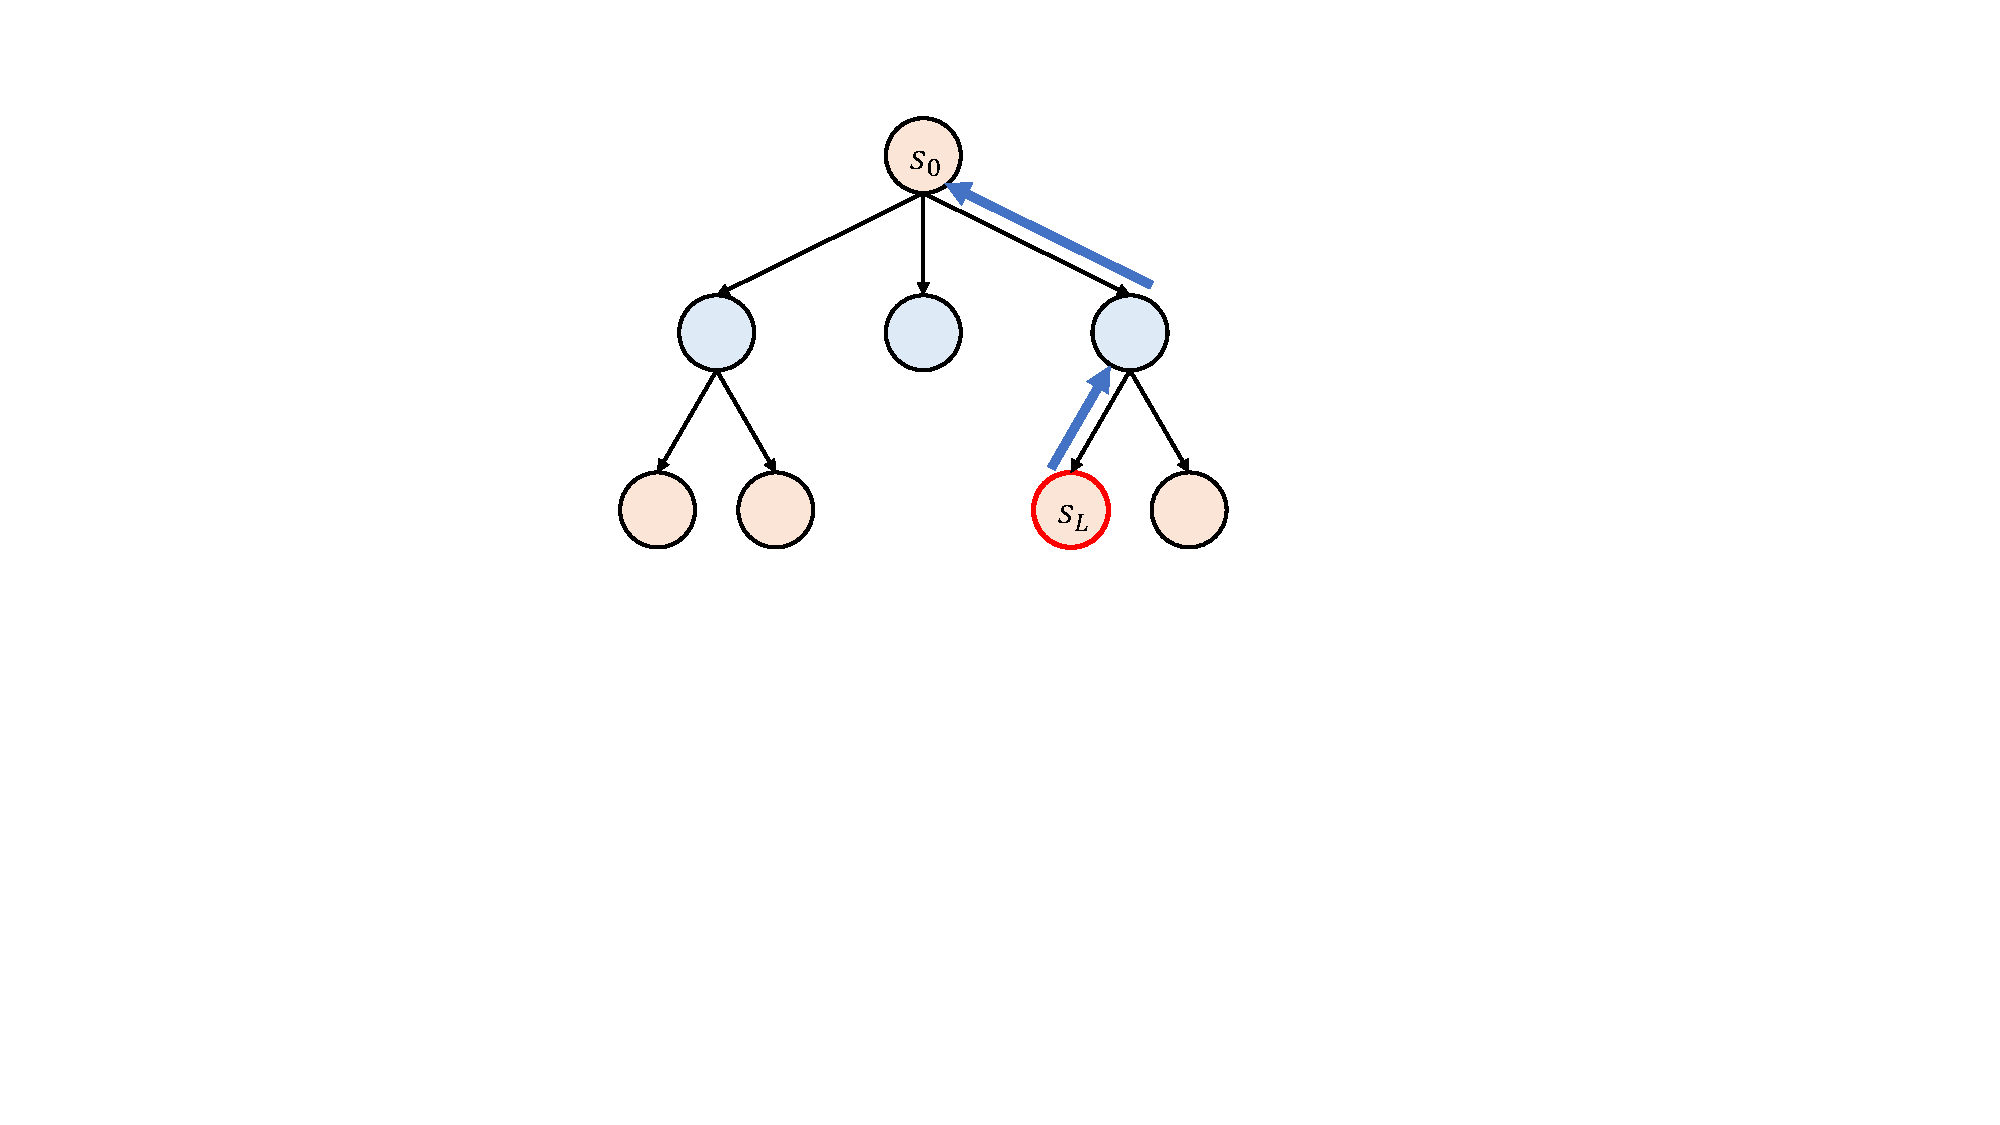
\includegraphics[width=\columnwidth]{figures/backpropagate_.pdf}
    \caption{逆伝播}
    \label{fig:backpropagate}
  \end{subfigure}
  \caption{MCTSの各ステップ~(オレンジ色のノードはdecisionノード, 青色のノードはchanceノード)}
  \label{fig:mcts}
\end{figure}

\subsubsection*{行動の決定方法}
一定回数のシミュレーションを行った後に, 実際に選ぶ行動を決定する.
根ノード$s_0$のそれぞれの子chanceノード$s_c$について, $N(s_c)^{1/\tau}$に比例した確率で子ノードを選択する.
選択した子ノードに対応するafterstateに遷移するような行動をとる.
$\tau$は温度パラメータと呼ばれ, $0$に近づくほど訪問回数に関して貪欲な選択をするようになる.
多様な学習データを集めるために学習の序盤では$\tau$を大きく設定し, 学習が進むについて$0$に近づける.

\subsubsection*{ニューラルネットワークの学習}
MCTSによるプレイによって得たデータを使ってニューラルネットワークを訓練する.
根ノード$s_0$をMCTSが評価する$n$ステップリターンを$z$とする.
これを方策・価値ニューラルネットワーク$f$の価値の出力$v$の学習ターゲットとする.
根ノード$s_0$から各子chanceノードへの訪問回数を正規化した確率分布を$\pmb{p}$とする.
これを方策・価値ニューラルネットワーク$f$の方策の出力$\pmb{\pi}$の学習ターゲットする.
よってまとめると式~\ref{eq:az_loss}で表される, 誤差関数$l$を最小化するようにパラメータを更新する.
afterstateを評価する価値ニューラルネットワーク$g$の学習も, $f$の価値関数の学習と同様に行う.
ただし実際の価値関数の学習においては付録~\ref{subsec:nn_impl}節で説明するように, 最小二乗誤差ではなくCross Entropy誤差を最小化するようにパラメータを更新する.
\begin{align}
\label{eq:az_loss}
l = (z-v)^2 - \pmb{p}^{\mathrm{T}} \log \pmb{\pi}
\end{align}

なお学習に使用するデータはPrioritized Experience Replay~\cite{prioritized}によってサンプルする.
Stochastic MuZeroは価値の予測誤差$|z-v|$をpriorityとした.

\subsection{先行研究の考察}
ここまでで2048の強化学習研究を概観した.
TD afterstate学習とAfterstate PPOはともに, 現在観測している状態からafterstateまでの遷移を内部で試行することを特徴とする.
またStochastic MuZero~(2048-AlphaZero)~はMCTSによる深いプランニングを行う.
よって現状2048で成果を出した手法はいずれも, 